\documentclass[aspectratio=169, 10pt]{beamer}

% Theme and Aesthetics
\usetheme{Madrid} 
\usecolortheme{dove} 
\usefonttheme{serif} 
\setbeamertemplate{navigation symbols}{} 
\setbeamertemplate{footline}[frame number]

% Packages
\usepackage{booktabs}
\usepackage{graphicx}
\usepackage{tikz}
\usetikzlibrary{shapes.geometric, arrows, positioning}
\usepackage{amsmath}
\usepackage{xcolor}

% Custom block styling - thick borders and taller boxes
\setbeamertemplate{blocks}[rounded][shadow=false]
\addtobeamertemplate{block begin}{%
    \setlength{\linewidth}{\dimexpr\linewidth-1pt\relax}%
}{}
\setbeamercolor{block title}{fg=black,bg=gray!30}
\setbeamercolor{block body}{fg=black,bg=gray!10}
\setbeamercolor{block title alerted}{fg=black,bg=gray!50}
\setbeamercolor{block body alerted}{fg=black,bg=gray!20}

% Thick border for blocks using mdframed
\usepackage{mdframed}
\surroundwithmdframed[linewidth=1.5pt, linecolor=black, backgroundcolor=gray!10, innertopmargin=10pt, innerbottommargin=10pt]{block}
\surroundwithmdframed[linewidth=3pt, linecolor=black, backgroundcolor=gray!20, innertopmargin=10pt, innerbottommargin=10pt]{alertblock}

% Presenter Notes Configuration
% Uncomment one of the following to enable notes:
% \setbeameroption{show notes on second screen=right}  % For dual-screen presentations
% \setbeameroption{show only notes}                     % To generate notes-only PDF
\setbeameroption{hide notes}                            % Default: hide notes in main PDF

% Title Info
\title{A Measurement Stack for Retail Media}
\author{Pranjal Rawat\inst{1} \and Muyang Ye\inst{2}}
\institute{\inst{1} 5th Year PhD Candidate, Georgetown University \and \inst{2} 3rd Year PhD Student, Georgetown University}
\date{}

\begin{document}

% Slide 1: Title
\begin{frame}[plain]
    \titlepage
\end{frame}

% =============================================================================
% INTRO SECTION
% =============================================================================

% Intro Slide 1: The Measurement Hierarchy
\begin{frame}{We Need an Econometric Measurement Stack\footnote{Similar to Marketing Mix Models (MMM) or GLM Risk Models, log-log demand models}}
    \centering
    \begin{columns}[t]
        \column{0.32\textwidth}
        \begin{block}{Accounting / ROAS}
            \centering
            Simple correlations \\
            \textit{biased}
        \end{block}

        \column{0.32\textwidth}
        \begin{alertblock}{Econometric Measurement $\star$}
            \centering
            Debiased Associations \\
            \textit{Elasticities}
        \end{alertblock}

        \column{0.32\textwidth}
        \begin{block}{Experiments}
            \centering
            Gold Standard \\
            \textit{expensive/difficult}
        \end{block}
    \end{columns}

    \vspace{0.5cm}
    \textbf{Why?} Traditional Accounting (ROAS) is likely biased and experimentation is expensive / difficult.
\end{frame}

% Intro Slide 2: The Data Pipeline (Visual)
\begin{frame}{Data Architecture}
    \centering
    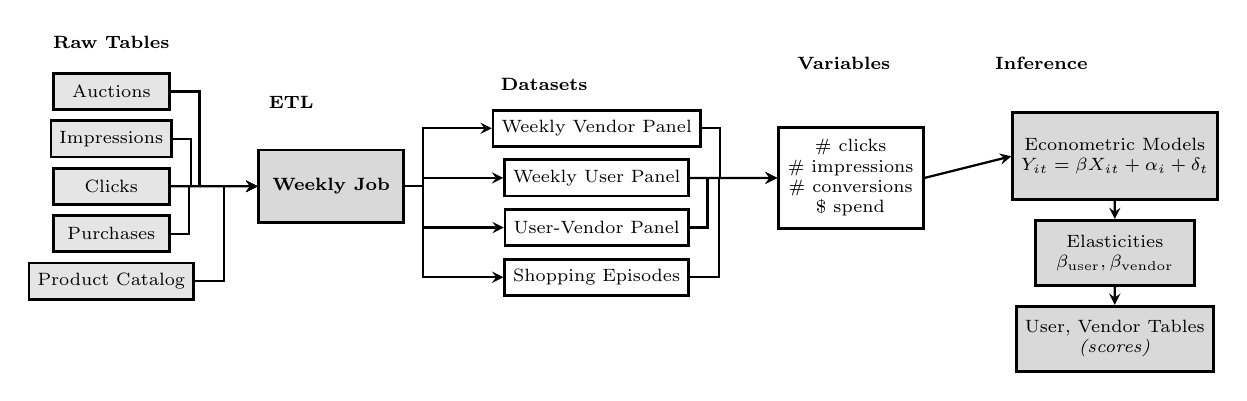
\begin{tikzpicture}[
        scale=0.92, transform shape,
        node distance=0.6cm,
        input/.style={rectangle, minimum width=1.6cm, minimum height=0.5cm, text centered, draw=black, line width=1pt, fill=gray!20, align=center, font=\scriptsize},
        process/.style={rectangle, minimum width=2cm, minimum height=1cm, text centered, draw=black, line width=1pt, fill=gray!30, align=center, font=\scriptsize},
        dataset/.style={rectangle, minimum width=2.4cm, minimum height=0.5cm, text centered, draw=black, line width=1pt, fill=white, align=center, font=\scriptsize},
        varbox/.style={rectangle, minimum width=2cm, minimum height=1.4cm, text centered, draw=black, line width=1pt, fill=white, align=center, font=\scriptsize},
        modelbox/.style={rectangle, minimum width=2.2cm, minimum height=0.6cm, text centered, draw=black, line width=1pt, fill=gray!30, align=center, font=\scriptsize},
        arrow/.style={thick,->,>=stealth}
    ]

        % Level 1: Raw Inputs (5 separate)
        \node (rawheader) [font=\bfseries\scriptsize] {Raw Tables};
        \node (auctions) [input, below=0.2cm of rawheader] {Auctions};
        \node (impressions) [input, below=0.12cm of auctions] {Impressions};
        \node (clicks) [input, below=0.12cm of impressions] {Clicks};
        \node (purchases) [input, below=0.12cm of clicks] {Purchases};
        \node (catalog) [input, below=0.12cm of purchases] {Product Catalog};

        % Level 2: Processing
        \node (etlheader) [right=1.2cm of impressions, yshift=0.5cm, font=\bfseries\scriptsize] {ETL};
        \node (etl) [process, right=1.2cm of clicks] {\textbf{Weekly Job}};

        % Level 3: The Outputs (Fan out)
        \node (datasetsheader) [right=1.2cm of etl, yshift=1.4cm, font=\bfseries\scriptsize] {Datasets};
        \node (vendor) [dataset, right=1.2cm of etl, yshift=0.8cm] {Weekly Vendor Panel};
        \node (user) [dataset, below=0.15cm of vendor] {Weekly User Panel};
        \node (uv) [dataset, below=0.15cm of user] {User-Vendor Panel};
        \node (session) [dataset, below=0.15cm of uv] {Shopping Episodes};

        % Level 4: Variables
        \node (varheader) [right=1.2cm of vendor, yshift=0.9cm, font=\bfseries\scriptsize] {Variables};
        \node (vars) [varbox, right=1.2cm of user] {\# clicks \\ \# impressions \\ \# conversions \\ \$ spend};

        % Level 5: Inference
        \node (inferheader) [right=1.2cm of varheader, font=\bfseries\scriptsize] {Inference};
        \node (models) [modelbox, minimum height=1.2cm, right=1.2cm of vars, yshift=0.3cm] {Econometric Models \\ $Y_{it} = \beta X_{it} + \alpha_i + \delta_t$};
        \node (effects) [modelbox, minimum height=0.9cm, below=0.25cm of models] {Elasticities \\ $\beta_{\text{user}}, \beta_{\text{vendor}}$};
        \node (storage) [modelbox, minimum height=0.9cm, below=0.25cm of effects] {User, Vendor Tables \\ \textit{(scores)}};

        % Arrows from inputs to ETL
        \draw [arrow] (auctions.east) -- ++(0.4,0) |- (etl.west);
        \draw [arrow] (impressions.east) -- ++(0.25,0) |- (etl.west);
        \draw [arrow] (clicks.east) -- (etl.west);
        \draw [arrow] (purchases.east) -- ++(0.25,0) |- (etl.west);
        \draw [arrow] (catalog.east) -- ++(0.4,0) |- (etl.west);

        % Arrows from ETL to outputs
        \draw [arrow] (etl.east) -- ++(0.25,0) |- (vendor.west);
        \draw [arrow] (etl.east) -- ++(0.25,0) |- (user.west);
        \draw [arrow] (etl.east) -- ++(0.25,0) |- (uv.west);
        \draw [arrow] (etl.east) -- ++(0.25,0) |- (session.west);

        % Arrows from outputs to variables
        \draw [arrow] (vendor.east) -- ++(0.25,0) |- (vars.west);
        \draw [arrow] (user.east) -- (vars.west);
        \draw [arrow] (uv.east) -- ++(0.25,0) |- (vars.west);
        \draw [arrow] (session.east) -- ++(0.4,0) |- (vars.west);

        % Arrow from variables to inference
        \draw [arrow] (vars.east) -- (models.west);
        \draw [arrow] (models.south) -- (effects.north);
        \draw [arrow] (effects.south) -- (storage.north);

    \end{tikzpicture}

    \vspace{0.3cm}
    \footnotesize
    \textit{Panels}: Repeated observations on same units (users, vendors). \\
    \textit{Shopping Episodes}: Defined by ``inactivity'' windows. \\
    \textit{Econometrics}: Statistical models connecting economic quantities.
\end{frame}

% =============================================================================
% CLICK EFFECTS SECTION
% =============================================================================
\section{Vendor Panels}

\begin{frame}[plain]
    \vfill
    \centering
    \Huge \textbf{Vendor Panels}
    \vfill
\end{frame}

% =============================================================================
% 1a-1b. STAGGERED DID (Callaway-Sant'Anna)
% =============================================================================
\begin{frame}{1a. Ads Drive Exposure but Don't Show Increases in Sales}
    \centering
    \textit{When vendors start advertising, what happens?}
    \vspace{0.2cm}

    \includegraphics[width=0.95\textwidth]{tabfig/event_study_unified_4panel.png}

    \vfill
    \rule{0.4\textwidth}{0.4pt} \\
    \scriptsize
    \textit{Callaway \& Sant'Anna (2021). 139k vendors, 26 weeks.} \\[2pt]
    $Y_{it} = \alpha_i + \lambda_t + \sum_e \theta_e \cdot \mathbf{1}\{t - G_i = e\} + \varepsilon_{it}$
\end{frame}

\begin{frame}{1b. Premium Vendors Seem to Benefit More}
    \centering
    \textit{Vendors with higher priced products, upon advertising, see more impressions.}

    \vspace{0.3cm}
    \textbf{By Price Tier}
    \vspace{0.3cm}

    \begin{tabular}{l r l}
        \toprule
        Segment & Effect & 95\% CI \\
        \midrule
        Premium & +0.3\%*** & [0.2, 0.4] \\
        Mid-tier & +0.2\%** & [0.1, 0.3] \\
        Budget & -0.1\% & [-0.3, 0.1] \\
        \bottomrule
    \end{tabular}

    \vfill
    \raggedright
    \rule{0.4\textwidth}{0.4pt} \\
    \scriptsize
    \textit{Effect = \% lift in impressions.} \\
    \textit{TWFE within segments.} \\
    \textit{Price tier = vendor's median product price quartile.}
\end{frame}

% =============================================================================
% 2a-2b. VENDOR PANEL (TWFE)
% =============================================================================
\begin{frame}{2a. Vendors Who Get More Clicks Also See More Sales}
    \begin{columns}[T]
        \begin{column}{0.45\textwidth}
            \vspace{0.2cm}
            \centering
            $\ln(\text{Sales}_{vw}) = \beta \ln(\text{Clicks}_{vw}) + \alpha_v + \delta_w + \varepsilon_{vw}$
            \vspace{0.3cm}

            \begin{tabular}{l r}
                \toprule
                Elasticity ($\beta$) & $\mathbf{0.64^{***}}$ \\
                SE & 0.003 \\
                95\% CI & [0.64, 0.65] \\
                $R^2_{\text{within}}$ & 0.07 \\
                \bottomrule
            \end{tabular}
        \end{column}
        \begin{column}{0.52\textwidth}
            \centering
            \includegraphics[width=\textwidth]{tabfig/beta_distribution_kde.png}

            \vspace{0.1cm}
            \scriptsize $\beta_v \sim N(0.64, 0.42)$
        \end{column}
    \end{columns}
    \vfill
    \raggedright
    \footnotesize
    \textit{$\ln(\text{Sales}_{vw}) = \beta \ln(\text{Clicks}_{vw}) + \alpha_v + \delta_w + \epsilon_{vw}$} \\
    \textit{Vendor-week panel with vendor ($\alpha_v$) and week ($\delta_w$) FE.} \\
    \textit{150k vendors, 26 weeks ($N=979k$). SE clustered by vendor.}
\end{frame}

\begin{frame}{2b. Some Vendors Stand to Benefit More from Clicks}
    \vspace{0.1cm}
    \footnotesize
    \begin{table}
        \centering
        \begin{tabular}{l l r}
            \toprule
            Dimension & Segment & Effect \\
            \midrule
            \textit{Price} & Premium ($>$\$82) & 0.00\% \\
             & Mid-High (\$40--82) & $\mathbf{+0.31\%}$ \\
             & Mid-Low (\$25--40) & -0.08\% \\
             & Budget ($<$\$25) & -0.10\% \\
            \midrule
            \textit{Activity} & Medium (Q3) & $\mathbf{+0.76\%}$ \\
             & High (Q4) & +0.39\% \\
             & Very High (Q5) & +0.04\% \\
            \bottomrule
        \end{tabular}
    \end{table}
    \normalsize

    \vspace{0.2cm}
    \centering
    \textit{Vendors who sell mid-high priced products and those with moderate prior activity see maximal impact of clicks on sales.}

    \vfill
    \raggedright
    \rule{0.4\textwidth}{0.4pt} \\
    \scriptsize
    \textit{TWFE by segment.} \\
    \textit{Price = vendor median product price quartile.} \\
    \textit{Activity = vendor's auction participation before first ad spend.}
\end{frame}

% =============================================================================
% USER-VENDOR PANEL SECTION
% =============================================================================
\section{User-Vendor Panel}

\begin{frame}[plain]
    \vfill
    \centering
    \Huge \textbf{User-Vendor Panel}
    \vfill
\end{frame}

% =============================================================================
% 3a-3b. USER-VENDOR-WEEK PANEL RESULTS
% =============================================================================
\begin{frame}{3a. Clicks Signal Browsing, Not Buying}

    $$ \text{Spend}_{uvt} = \beta \cdot \text{Clicks}_{uvt} + \text{FE} + \epsilon $$

    \begin{center}
    \begin{tabular}{l r r}
        \toprule
        Specification & $\beta$ & p \\
        \midrule
        OLS (no FE) & $+0.22$ & 0.08 \\
        + User FE & $+0.25$ & 0.06 \\
        \midrule
        + Vendor FE & $-0.20$ & 0.23 \\
        + User + Week + Vendor FE & $-0.23$ & 0.36 \\
        \bottomrule
    \end{tabular}
    \end{center}

    \vfill
    \raggedright
    \rule{0.4\textwidth}{0.4pt} \\
    \scriptsize
    \textit{User-vendor-week panel: 1,544 users, 18,603 vendors, 26 weeks (N=28,619). SE clustered by user.} \\
    \textit{Clicks: 85\% have C=1, 12\% have C=2, 3\% have C$\geq$3. 42 rows with C=0 (organic/prior-week).} \\
    \textit{Spend: 99.2\% have zero spend. 235 purchases (0.8\%). Median \$15, mean \$35, range \$4--\$499.}

    \note{
        \textbf{Data:} User-Vendor-Week panel with 28,619 rows. 1,544 unique users, 18,603 unique vendors, 26 weeks. Extremely sparse: 99.2\% zero spend, only 235 purchases (0.8\%). Clicks distribution: 85\% have C=1, 12\% have C=2, 3\% have C$\geq$3. Spend distribution: Median \$15, mean \$35, range \$4--\$499.

        \textbf{Model:} Unit of analysis is the (user, vendor, week) triple. Y = dollar spend on vendor v by user u in week t. C = count of sponsored clicks. Standard errors clustered by user.

        \textbf{Key finding:} OLS shows positive association (users who click more tend to spend more). But adding Vendor FE flips the sign to negative. This is the critical insight.

        \textbf{Why the flip?} Selection bias---users click on vendors they are already interested in. Within vendor, more clicks = comparison shopping / browsing, not buying intent.

        \textbf{Statistical significance:} None of the estimates are significant (all p $>$ 0.05). The effect is economically and statistically indistinguishable from zero.

        \textbf{Takeaway:} Clicks signal browsing behavior, not purchase intent. The positive raw correlation is driven entirely by selection.

        \textit{Source: shopping-episode/archive/run\_regressions.py}
    }
\end{frame}

\begin{frame}{3b. Repeated Clicks on Same Vendor Signals Strong Intent}

    $$ \text{Spend}_{uvt} = \beta \cdot \text{Clicks}_{uvt} + \text{FE} + \epsilon \quad \text{(subset regressions)} $$

    \begin{center}
    \begin{tabular}{l r r r}
        \toprule
        Segment & N & $\beta$ & p \\
        \midrule
        Single click (C=1) & 24,303 & $-44.5$ & 0.001* \\
        Repeat click (C$\geq$2) & 4,316 & $+0.26$ & 0.63 \\
        \midrule
        Low rank (rank $>$ 3) & 20,983 & $-0.34$ & 0.29 \\
        Top rank (rank $\leq$ 3) & 7,636 & $+0.69$ & 0.43 \\
        \midrule
        Niche vendor & 27,283 & $-0.45$ & 0.28 \\
        Popular vendor & 1,336 & $+0.05$ & 0.78 \\
        \bottomrule
    \end{tabular}
    \end{center}

    \vfill
    \raggedright
    \rule{0.4\textwidth}{0.4pt} \\
    \scriptsize
    \textit{Each row is a separate regression on that subset.} \\
    \textit{Repeat = 2+ clicks same vendor/week. Top rank = avg rank $\leq$ 3. Popular = 11+ total clicks.}

    \note{
        \textbf{Data:} Same panel as 3a. Each row in the table is a separate regression on that segment only.

        \textbf{Single vs Repeat clicks:} Single clicks strongly negative ($-44.5$, p=0.001), repeat clicks positive ($+0.26$, p=0.63). Single click = casual browsing. Repeat clicks = deliberate interest in that vendor.

        \textbf{Rank position:} Top-rank clicks more positive ($+0.69$) than low-rank ($-0.34$). Top rank ads get more qualified/intentional clicks.

        \textbf{Vendor popularity:} Niche vendors see negative effect ($-0.45$), popular vendors near zero ($+0.05$). Niche vendors: clicking = discovery/browsing. Popular vendors: clicking = targeted search.

        \textbf{Comparison Shopping Evidence:} Converters click 9.1 times on average vs 1.0 for non-converters. Converters click on 4.2 vendors vs 1.1 for non-converters. Converters click 9x more than non-converters and click on 4x more vendors.

        \textbf{Takeaway:} Heavy clicking = comparison shopping before buying. Heterogeneity exists---repeat clicks and top-rank clicks are different from single/low-rank clicks.

        \textit{Source: shopping-episode/archive/run\_segmentation.py}
    }
\end{frame}

\begin{frame}{3c. Users Seem to Respond to Clicks Differently}

    $$ Y_{uvt}^{\text{dm}} = \beta_u \cdot C_{uvt}^{\text{dm}} + \epsilon, \quad \beta_u = \bar{\beta} + b_u $$

    \vspace{0.1cm}
    \scriptsize Vendor-demeaned model. $\bar{\beta}$ = population average, $b_u$ = user-specific deviation.
    \normalsize

    \begin{columns}[T]
        \begin{column}{0.48\textwidth}
            \centering
            \includegraphics[width=\textwidth]{tabfig/user_slopes_kde.png}
        \end{column}
        \begin{column}{0.48\textwidth}
            \vspace{0.5cm}
            \begin{tabular}{l r}
                \toprule
                Population avg $\bar{\beta}$ & $-0.16$ \\
                \midrule
                $\beta_u > 0$ & 8.5\% \\
                $\beta_u < 0$ & 91.5\% \\
                \midrule
                Mean $\beta_u$ & $-0.16$ \\
                Std $\beta_u$ & 3.11 \\
                \bottomrule
            \end{tabular}

            \vspace{0.3cm}
            \small
            \textit{User heterogeneity is real, but most users show negative relationship.}
        \end{column}
    \end{columns}

    \vfill
    \raggedright
    \rule{0.4\textwidth}{0.4pt} \\
    \scriptsize
    \textit{Mixed effects model with vendor FE (via demeaning) and user random slopes.} \\
    \textit{$Y^{\text{dm}} = Y - \bar{Y}_v$, $C^{\text{dm}} = C - \bar{C}_v$. N=28,619. 1,544 users.}

    \note{
        \textbf{Data:} Same panel. Mixed effects model with vendor FE (via demeaning) and user random slopes.

        \textbf{Model:} $Y^{dm} = Y - \bar{Y}_v$ (vendor-demeaned spend). $C^{dm} = C - \bar{C}_v$ (vendor-demeaned clicks). $\bar{\beta}$ = population average effect. $b_u$ = user-specific deviation (random effect). $\beta_u$ = user-specific slope.

        \textbf{Why demeaning?} 18,603 vendors = too many dummy variables for mixed effects estimation. Demeaning absorbs vendor FE equivalently (Frisch-Waugh-Lovell theorem). Then fit mixed effects with user random slopes on demeaned data.

        \textbf{Results:} Population average $\bar{\beta} = -0.16$ (similar to pyfixest Full FE: $-0.23$). 8.5\% of users show $\beta_u > 0$. 91.5\% of users show $\beta_u < 0$. Mean $\beta_u = -0.16$, Std $\beta_u = 3.11$. Model converged successfully.

        \textbf{Interpretation:} Most users (91.5\%) show negative click-spend relationship. Wide heterogeneity exists (Std = 3.11). Small minority (8.5\%) where clicks do predict spending.

        \textbf{Takeaway:} User heterogeneity is real, but most users show negative relationship.

        \textbf{Narrative Arc (3a $\rightarrow$ 3b $\rightarrow$ 3c):} (1) Overall, clicks don't cause purchases. Vendor FE flips the sign. (2) But there's heterogeneity---repeat clicks and top-rank clicks are different. Converters click way more (comparison shopping). (3) User-level analysis confirms heterogeneity exists, but 92\% of users still show negative relationship.

        \textbf{Bottom line:} Clicks are a signal of shopping intent, not a cause of purchases. Users who buy click a lot, but clicking doesn't make them buy.

        \textit{Source: shopping-episode/archive/mixed\_effects\_converged\_results.txt}
    }
\end{frame}

% =============================================================================
% 4. AD RANK --> CLICKS (Muyang)
% =============================================================================
\section{Ad Impressions}

\begin{frame}[plain]
    \vfill
    \centering
    \Huge \textbf{Ad Impressions}
    \vfill
\end{frame}

\begin{frame}{4a. Higher-Ranked Ads Associated with Higher CTR}
\[
\mathbb{E}[\text{clicked} \mid \text{rank}]
= \beta_0 - \beta_1 \cdot \text{rank} + \text{controls}.
\]
\vspace{0.8em}

\begin{table}[ht]
\centering
\begin{tabular}{lcccc}
\hline
Method & Baseline OLS & Vendor FE & Vendor + Time FE & DML \\
\hline
Change ($-\beta_1$) & +0.0023pp & +0.0041pp & +0.0036pp & +0.0184pp \\
vs. baseline (2.8\%) & +0.08\% & +0.15\% & +0.13\% & +0.66\% \\
\hline
\end{tabular}
\end{table}

\vfill
\rule{0.3\textwidth}{0.4pt} \\
\scriptsize
\textit{Rank $\in [1, 50]$ (1 = top). Clicked $\in \{0,1\}$. Unit = 1 ad impression. FE controls for time-invariant heterogeneity. DML uses ML to control confounding.}

\end{frame}

\begin{frame}{4b. Jump in CTR at Display Cutoffs}
    \centering
    Cutoff at rank 2: \textbf{+0.189pp} (+6.9\%)

    \begin{figure}
        \centering
        \includegraphics[width=0.4\linewidth]{tabfig/rdd.png}
    \end{figure}

\vfill
\rule{0.3\textwidth}{0.4pt} \\
\scriptsize
\textit{Display shows 4 ads per row. ``Crossing'' = improving from just below to just above a row boundary (e.g., rank 5 $\rightarrow$ 4). Crossing helps at top (ranks 2, 4), hurts at bottom (ranks 10, 12).}

\end{frame}

\begin{frame}{4c. User Attention Concentrated in Middle Positions}
    \begin{figure}
        \centering
        \includegraphics[width=0.85\linewidth]{tabfig/rankbin.png}
    \end{figure}

\vfill
\rule{0.3\textwidth}{0.4pt} \\
\scriptsize
\textit{Possible mechanisms: (1) Discovery of high-quality products in middle slots, (2) Users avoid top ads (ad blindness) and engaged users scroll deeper.}

\end{frame}

\begin{frame}{4d. Higher Quality Vendors Less Sensitive to Ranking}

\begin{figure}
    \centering
    \includegraphics[width=0.9\linewidth]{tabfig/vendor.png}
\end{figure}

\vfill
\rule{0.3\textwidth}{0.4pt} \\
\scriptsize
\textit{Medium-quality vendors most sensitive to ranking. High-quality vendors attract clicks regardless of position. N=291 vendors with $\geq$100 impressions across $\geq$3 rank positions.}

\end{frame}

\begin{frame}{Takeaways}
    \begin{enumerate}
        \item When vendors start advertising, clicks rise but sales do not (immediately) show an increase
        \vspace{0.4cm}
        \item However, vendors who receive more clicks also see more sales (association)
        \vspace{0.4cm}
        \item Yet, a particular user clicking more on a vendor does not imply they will spend on it; they may simply be browsing or uncertain
        \vspace{0.4cm}
        \item In general top ranked ads do better, but there seems to be a few middle ranks that get even more clicks
        \vspace{0.4cm}
        \item In all these findings, one can find segments of users or vendors that stand out
    \end{enumerate}
\end{frame}

\begin{frame}[plain]
    \vfill
    \centering
    \Huge \textbf{What do you think?}

    \vspace{1cm}
    \Large Thank you, Abelino! :)
    \vfill
\end{frame}

\end{document}
